\section{Data Pre-processing}
The dataset utilized in this study is derived from a CSV file containing comprehensive specifications of Intel CPUs. This dataset serves as the foundation for our analysis, providing detailed information on various CPU features that are essential for understanding clock speed trends. In this section, we describe the dataset's structure, contents, and the relevance of its attributes to our study.

\subsection{Dataset Overview}
The CSV file comprises numerous rows, each representing an individual Intel CPU model. Each row contains multiple attributes describing the specifications and characteristics of the CPU. The dataset encompasses a diverse range of CPU models across different series, generations, and intended applications (e.g., consumer desktops, laptops, server-grade CPUs), ensuring a comprehensive coverage of CPU types and their respective attributes.

\subsection{Data Relevance and Usefulness}
The following attributes from the dataset are particularly relevant for analyzing CPU clock speeds:

\begin{itemize}
    \item \textbf{Processor\_Base\_Frequency}: This attribute represents the base clock speed of the CPU, measured in gigahertz (GHz). Higher base frequencies generally indicate faster processing capabilities and overall performance.
    \item \textbf{Max\_Turbo\_Frequency}: Many modern CPUs support Turbo Boost technology, which dynamically increases the clock speed under certain conditions. This attribute specifies the maximum Turbo Boost frequency achievable by the CPU, providing insights into its potential performance capabilities.
    \item \textbf{nb\_of\_Cores}: The number of cores in a CPU impacts its ability to handle multiple tasks simultaneously. CPUs with more cores can potentially support higher clock speeds under optimal conditions, affecting overall performance trends.
    \item \textbf{nb\_of\_Threads}: This attribute represents the number of threads supported by the CPU, which is often influenced by technologies like Intel's Hyper-Threading. A higher number of threads can contribute to better resource utilization and potentially higher effective clock speeds for certain workloads.
    \item \textbf{TDP (Thermal Design Power)}: The TDP indicates the maximum amount of heat the CPU cooling system needs to dissipate. This attribute is closely related to the CPU's power consumption and thermal characteristics, which can impact clock speed potential and performance.
    \item \textbf{Lithography}: This attribute refers to the manufacturing process node (e.g., 14nm, 10nm) used in producing the CPU. Advancements in manufacturing processes can lead to higher clock speeds and improved efficiency in newer CPU generations.
\end{itemize}

Our objective is to analyze historical trends in CPU clock speeds using these attributes. Understanding how clock speeds have evolved across different CPU generations, architectural improvements, and technological shifts is crucial for identifying patterns and making informed predictions. By focusing on these critical attributes, we aim to uncover insights into the factors driving CPU clock speed improvements and contributing to the overall technological progress in CPU development.

\subsection{Load Data}
In this section, we load and clean the data for our analysis.

\begin{lstlisting}[language=R]
    # Load necessary library
    library (dplyr)

    # Importing data
    intel_cpu <- read.csv ("../data/Intel_CPUs.csv")

    # Specify the desired columns
    desired_cols <- c ("Processor_Base_Frequency", "nb_of_Cores", "nb_of_Threads", "TDP", "Lithography")

    # Subset the data to only include the desired columns
    intel_cpu_subset <- intel_cpu %>% select (one_of(desired_cols))

    # Remove rows with base frequency measured in MHz
    intel_cpu_subset <- intel_cpu_subset %>%
        filter (!grepl ("MHz", Processor_Base_Frequency))

    # Convert necessary columns to appropriate types if they are not
    # Removing 'GHz' and converting Processor_Base_Frequency to numeric
    intel_cpu_subset$Processor_Base_Frequency <- 
        as.numeric (gsub (" GHz", "", intel_cpu_subset$Processor_Base_Frequency))

    # Additional conversion to ensure nb_of_Cores, nb_of_Threads, TDP, and Lithography are numeric where applicable
    intel_cpu_subset$nb_of_Cores <- 
        as.numeric (intel_cpu_subset$nb_of_Cores)
    intel_cpu_subset$nb_of_Threads <- 
        as.numeric (intel_cpu_subset$nb_of_Threads)
    intel_cpu_subset$TDP <- 
        as.numeric (gsub (" W", "", intel_cpu_subset$TDP))
    intel_cpu_subset$Lithography <- 
        as.numeric (gsub (" nm", "", intel_cpu_subset$Lithography))

\end{lstlisting}

\vspace*{1cm}

\subsection{Handling missing values}

First, we reselect among the originally selected data columns so as to minimize missing data. So far, we have selected 6 columns as explained in the above section. After this consideration, we have removed the column Max\_Turbo\_Frequency, due to it having a very limited amount of data points especially in correspondence to older CPU processors.\\

Then, we employed listwise deletion to remove cases of missing or bad data. We could have chosen other similar methods like mean imputation, median imputation or regression imputation, and in truth these methods have their own pros and cons. What led us to choose listwise were based on context:
\begin{itemize}
    \item We wanted to quickly prototype our programs. Implementation of listwise deletion is quick and simple.
    \item We wanted a neutral algorithm. Unlike methods like regression imputation, this does not introduce sample bias.
\end{itemize}

In contrast and for example, here's why using median imputation is not suitable for our attributes and why removing rows with missing values is a better approach:
\begin{itemize}
    \item Processor\_Base\_Frequency:
    \begin{itemize}
        \item Contextual Integrity: The base frequency is a critical performance metric measured in GHz. Imputing a median value may introduce inaccuracies because the actual base frequencies are often specific to CPU models and designs. These values are precise and need to reflect the true performance characteristics of the CPU.
        \item Range and Units: Base frequencies vary within specific ranges, and a median value might not accurately represent the operational characteristics of the CPUs, especially when considering variations in architecture and generation.
    \end{itemize}

    \item nb\_of\_Cores and nb\_of\_Threads:
    \begin{itemize}
        \item Specific Configuration: The number of cores and threads is an intrinsic property of a CPU model, determined by its design and intended use. These are exact numbers that are integral to the CPU's capability. Imputing a median would mean assigning an arbitrary number of cores or threads that do not exist in the actual hardware configurations, leading to misleading results.
        \item Consistency: Each CPU model has a specific number of cores and threads. Removing rows with missing values ensures we only analyze data with complete and accurate configurations.
    \end{itemize}

    \item TDP (Thermal Design Power):
    \begin{itemize}
        \item Thermal Characteristics: TDP is a precise measure of the maximum heat a CPU can generate under typical load, directly influencing cooling solutions and performance. Using a median TDP might not accurately reflect the thermal design considerations specific to different CPU models.
        \item Power Management: Different CPUs have different power and thermal characteristics. It's crucial to work with exact TDP values to maintain the accuracy of the analysis.
    \end{itemize}

    \item Lithography:
    \begin{itemize}
        \item Manufacturing Process: Lithography measures the process technology node (e.g., 14nm, 10nm). These are fixed and precise values associated with the manufacturing process of the CPU. A median value would not accurately represent any actual process node and could distort the analysis of technological trends.
    \end{itemize}
\end{itemize}

\begin{lstlisting}[language=R]
    # Remove rows with missing values in the specific columns
    cols_to_check <- c ("Processor_Base_Frequency", "nb_of_Cores", "nb_of_Threads", "TDP", "Lithography")
    intel_cpu_subset <- intel_cpu_subset[complete.cases (intel_cpu_subset[, cols_to_check]), ]

    # Display the resulting subset
    print (intel_cpu_subset)
\end{lstlisting}

\subsection{Handling outliers}
Certain data points in the column TDP (Thermal Design Power) are extreme compared to others in the same column. These values are outliers. In the below figures, they are seen as the lone tall spikes.\\

Outliers in our dataset can have both positive and negative implications. Outliers can bring out the true nature of our sample population, in which case we should retain these values. Outliers can also mean experimental errors, affecting the integrity and accuracy of our data analysis, in which case we should correct or remove these values.\\

In this assignment we have chosen to correct outlier values. We will employ log transformation. Log transformation simply means applying a base-10 logarithm function to a column. This should correct the data points at certain columns by re-adjusting data points the more that are far away from 0. Specifically, we will transform the column TDP where most assumably erroneous outliers occurred:
\begin{lstlisting}[language=R]
    intel_cpu_temp <- intel_cpu_subset
    intel_cpu_temp$TDP <- log10(intel_cpu_temp$TDP)
\end{lstlisting}

\begin{figure}[H]
    \begin{center}
    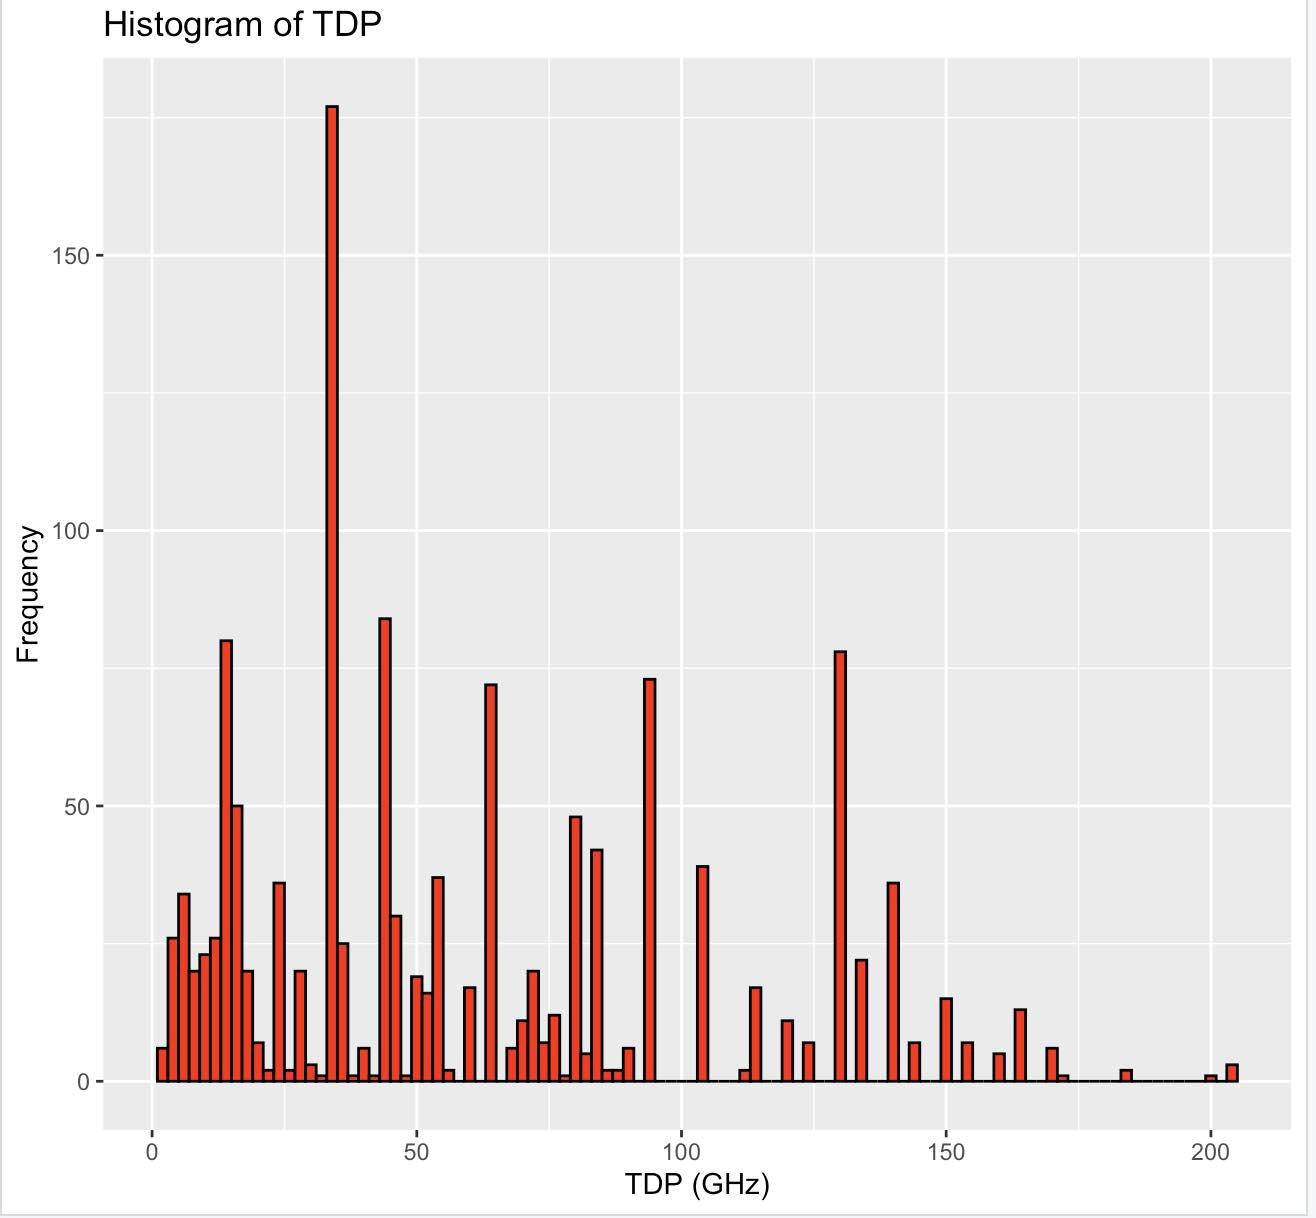
\includegraphics[width=14cm]{graphics/tdp_log_before.png}
    \end{center}
\end{figure}

\begin{figure}[H]
    \begin{center}
    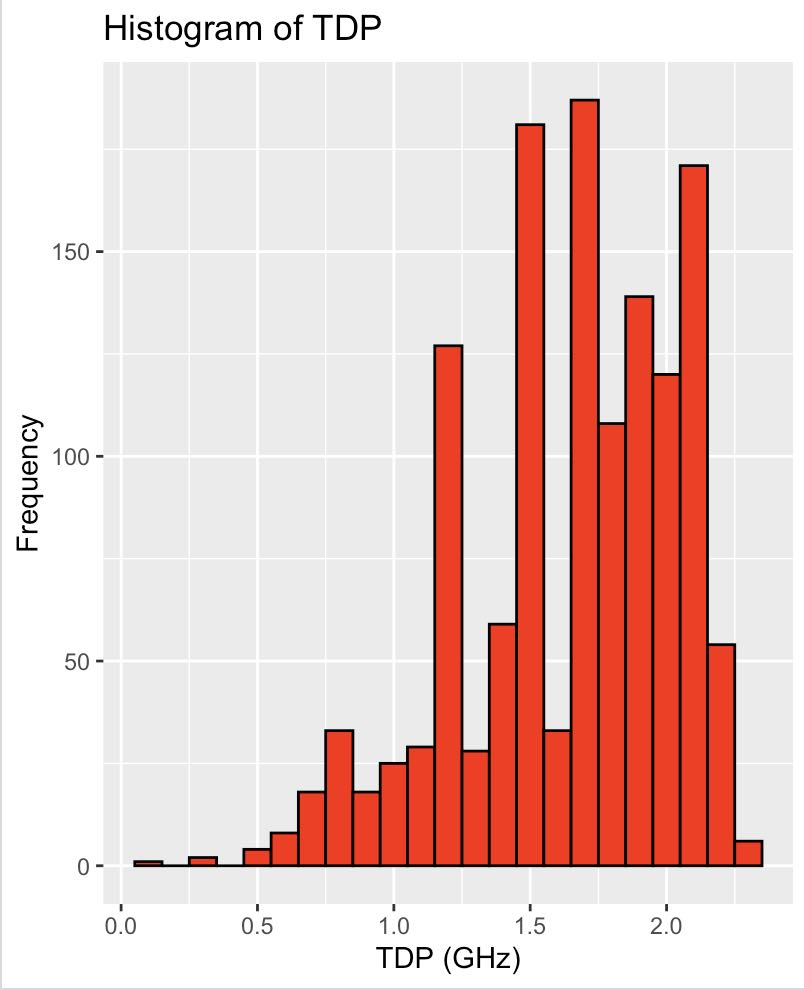
\includegraphics[width=14cm]{graphics/tdp_log_after.png}
    \end{center}
\end{figure}

\newpage